\section{Frontend des Web-Editors}\label{sec:editor-frontend}
Nachdem die erste Hälfte der Implementierung durch fulibWorkflows abgeschlossen ist, konzentrieren sich dieses und das folgende Kapitel um den dazugehörigen Web-Editor.
Der Web-Editor besteht aus einem Frontend und einem Backend, welche beide über Heroku deployt wurden und somit\footnote{unter \url{https://workflows-editor-frontend.herokuapp.com/}}
erreichbar sind.

\begin{figure}[h]
    \centering
    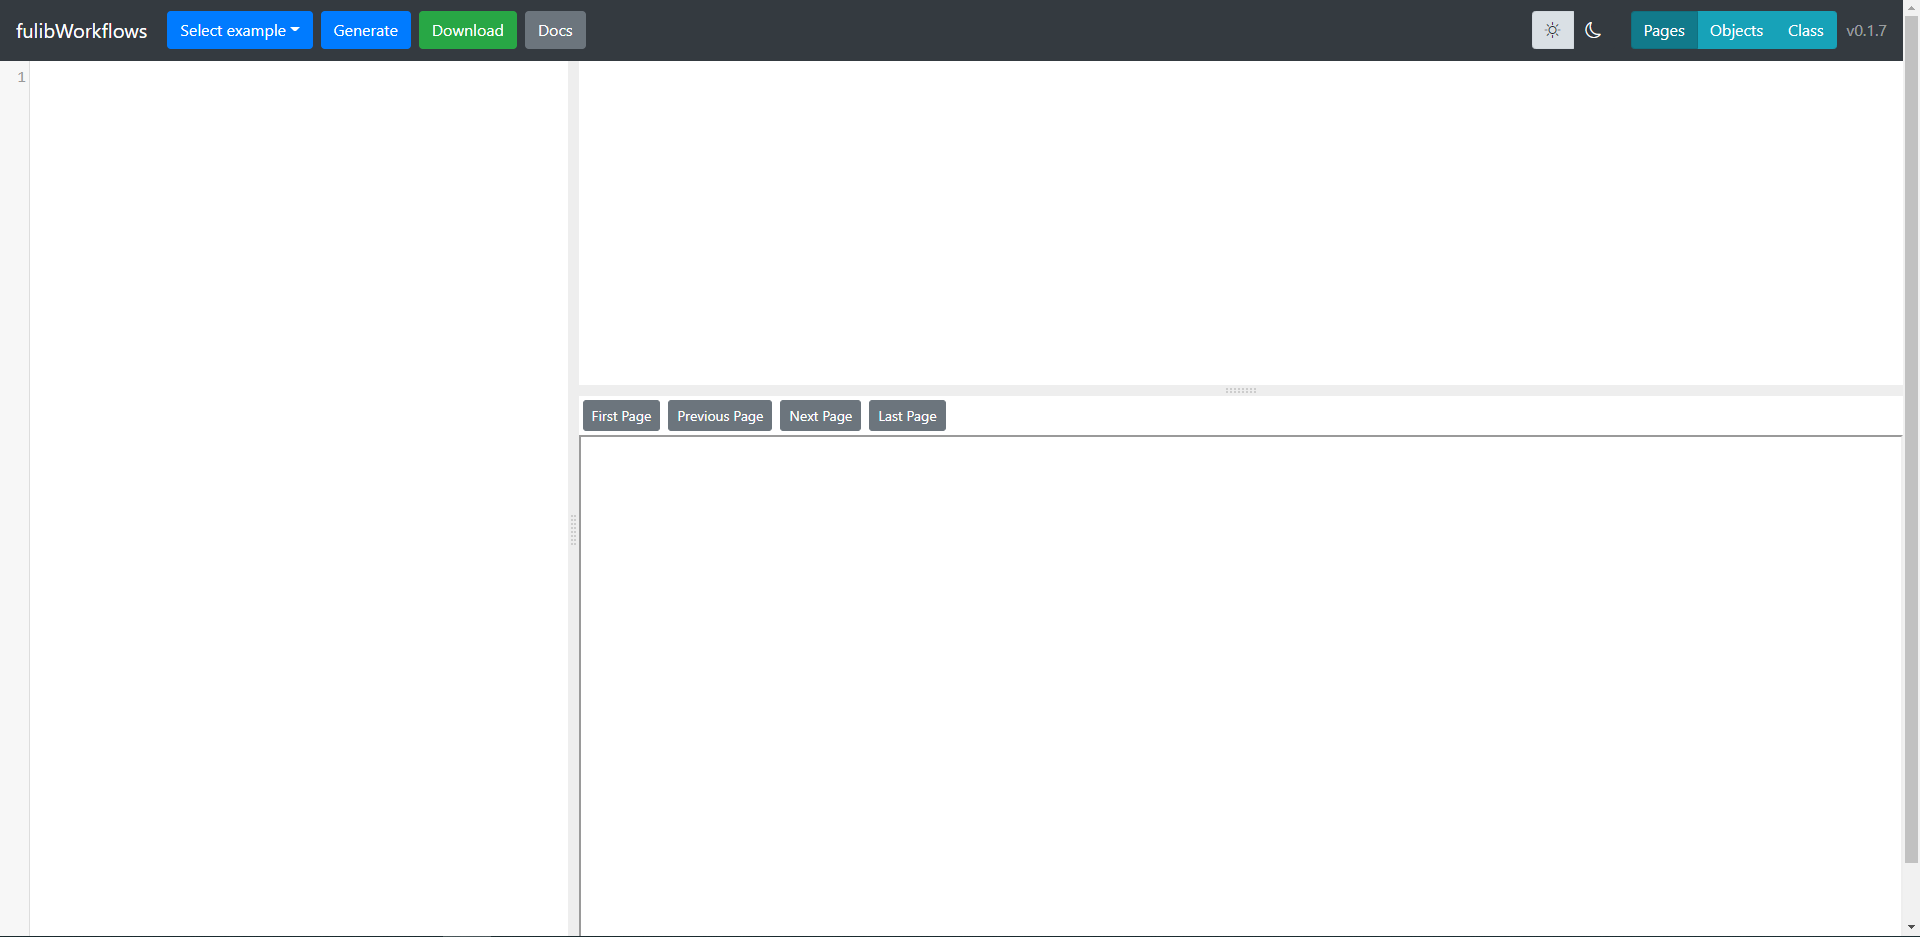
\includegraphics[width=1.0\textwidth]{images/3.2/workflows-complete}
    \caption{Oberfläche des Web-Editors für fulibWorkflows}
    \label{fig:frontend}
\end{figure}

In Abbildung~\ref{fig:frontend} ist die Oberfläche des Web-Editors dargestellt.
Dieser besteht aus vier verschiedenen Bereichen.
Der erste dieser Bereiche ist die Navigationsleiste, welche den oberen Rand der Oberfläche einnimmt.
In dieser existieren zuerst, von links nach rechts, zwei Buttons, welche das Theme des Code-Editors abändern.
Damit ist es möglich einen Light- oder Dark-Mode zum Schreiben des Codes zu verwenden.
Danach folgt ein Dropdown-Menü, mit welchem es möglich ist verschiedene vorgefertigte Beispiele zu laden.
Das ausgewählte Beispiel wird automatisiert nach der Auswahl ans Backend geschickt und dort generiert, sodass nach einer kurzen Wartezeit ein \ac{ES}-Board und falls
vorhanden Mockups und Diagramme angezeigt werden können.
Als Nächstes folgt ein Knopf zum Anstoßen einer Generierung, nachdem dieser Knopf gedrückt wurde und die Generierung angestoßen ist, erscheint ein Ladekreis in dem Knopf,
um als Indikator dafür zu dienen, dass der Prozess noch nicht abgeschlossen ist.
Die Web-Anwendung ermöglicht es zusätzlich die in der Oberfläche erstellten Dateien herunterladen.
Hierfür öffnet sich ein Pop-Up, nachdem der Download-Knopf betätigt wurde.
Dieses Fenster ist in Abbildung~\ref{fig:download} dargestellt.

\begin{figure}[h]
    \centering
    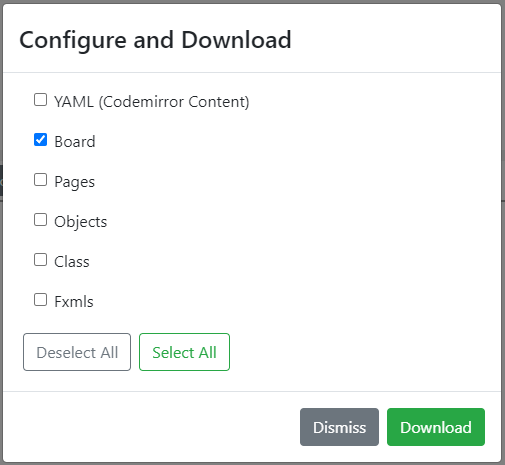
\includegraphics[width=0.5\textwidth]{images/3.2/download}
    \caption{Download-Fenster}
    \label{fig:download}
\end{figure}

Im sich öffnenden Fenster erhält der Benutzende die Möglichkeit auszuwählen, welche Dateien heruntergeladen werden sollen.
Es können einzelne Dateien heruntergeladen werden, wie der Inhalt des Code-Editors, das generierte \ac{ES}-Board oder aber alle Dateien
die durch die aktuelle Workflow-Beschreibung im Code-Editor generiert wurden.
Mit einem Klick auf den Download-Knopf, welcher sich neben dem Dismiss-Knopf befindet, wird eine Zip-Datei generiert und automatisch durch den jeweiligen Browser heruntergeladen.

Für den Fall, dass der Nutzende noch keine Erfahrungen mit der Syntax von fulibWorkflows gemacht hat, kann die Dokumentation, welche auf Englisch verfasst ist, mit einem Klick
auf den grauen Docs-Knopf aus Abbildung~\ref{fig:frontend} geöffnet werden.
Die Dokumentation stammt aus dem GitHub-Repository von fulibWorkflows.
Letztlich befindet sich ganz rechts die aktuelle Versionsnummer des Web-Editors.

\subsection{Code-Editor}\label{subsec:codeeditor}
In diesem Kapitel wird der Code-Editor, welcher das Herzstück der Anwendung ist, erläutert.
Dieser befindet sich auf der linken Seite der in Abbildung~\ref{fig:frontend} dargestellten Oberfläche.
Wie zuvor bereits beschrieben wurde hierbei ein Codemirror verwendet.
Durch die Verwendung der \textit{ngx-codemirror} Bibliothek vereinfacht sich das Einbinden eines Codemirrors in eine Angular-Anwendung.
Dadurch kann eine Konfiguration des Codemirrors über ein Options-Objekt übergeben werden.
Die Konfiguration des Codemirrors ist in Listing~\ref{listing:configuration} dargestellt.

\begin{listing}[!ht]
    \inputminted[firstnumber=49]{ts}{listings/3.2/codemirror-options.ts}
    \caption{Codemirror-Konfiguration}
    \label{listing:configuration}
\end{listing}

In Zeile 50 werden die Zeilennummern am linken Rand des Codemirrors aktiviert.
Das aktuelle Theme wird in der folgenden Zeile ebenfalls übergeben.
Da es zwei verschiedene Themes gibt, welche verwendet werden können, wird der Wert aus einer weiteren Variable übernommen.
Codemirror stellt bereits zahlreiche verschiedene Themes für Light-Mode oder Dark-Mode bereit.
Initial wird der Codemirror mit dem Light-Theme geladen, das Umstellen des Themes erfolgt über die entsprechenden Knöpfe in der Navigationsleiste, wie bereits zuvor beschrieben.
Abbildung~\ref{fig:themes} zeigt den Codemirror in beiden Modi, wobei sich sowohl Light- als auch Dark-Mode nah an den Standard-Modi von IntelliJ orientieren.

% Diese Abbildungen ggf. in den Anhang verschieben
\begin{figure}%
    \centering
    \subfloat[\centering Light-Theme]{{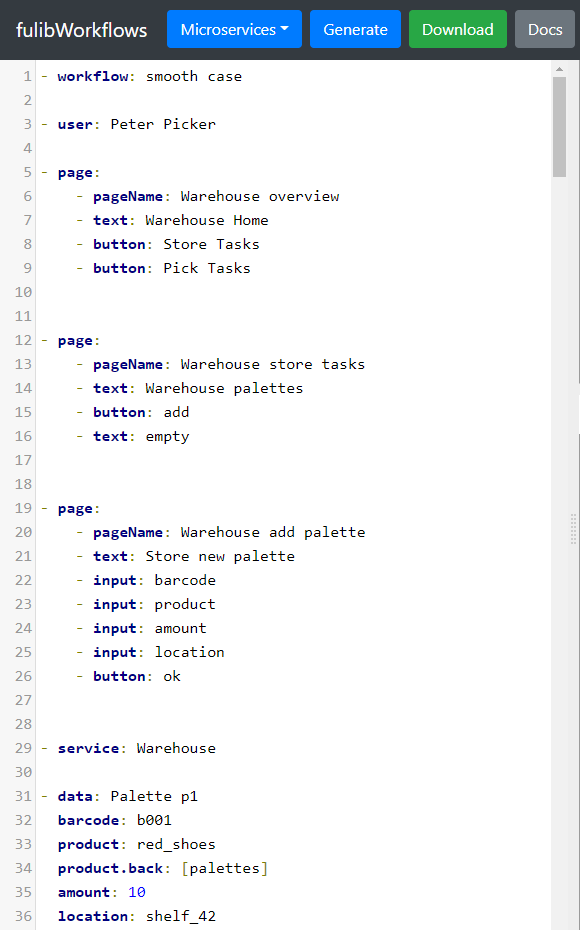
\includegraphics[width=4cm,height=6cm]{images/3.2/light-theme} }}%
    \qquad
    \subfloat[\centering Dark-Theme]{{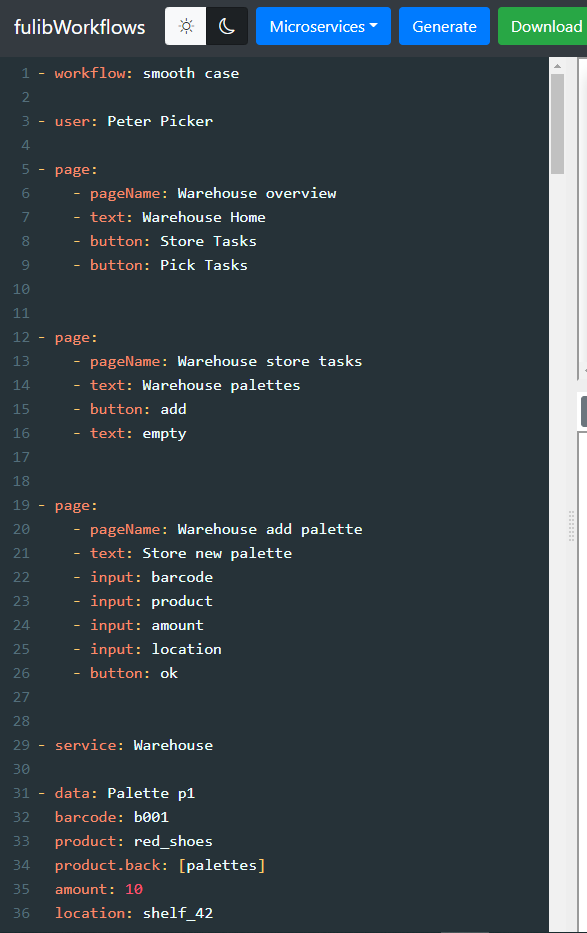
\includegraphics[width=4cm,height=6cm]{images/3.2/dark-theme} }}%
    \caption{Themes des Codemirrors}%
    \label{fig:themes}%
\end{figure}

In Zeile 52 aus Listing~\ref{listing:configuration} wird die Programmiersprache des Editors festgelegt.
Da die Workflow-Beschreibungen von fulibWorkflows in \textit{.es.yaml}-Dateien angelegt/gespeichert werden, wird die Programmiersprache auf \textit{yaml} festgelegt.
Dieser Modus wird von Codemirror selbst bereitgestellt und bedarf zur Verwendung einen Import in der \textit{main.ts}-Datei der Angular-Anwendung.
Über die Option \textit{extraKeys} können Tasten oder Tastenkombinationen an weitere Funktionen gekoppelt werden.
In Zeile 54 wird das Öffnen einer Liste an vorgeschlagenen Wörtern geöffnet, nachdem der Nutzende die Tastenkombination ``Strg+Leertaste'' gedrückt hat.
Damit dies funktioniert, benötigt es das Importieren des \textit{show-hint}-AddOns von Codemirror in der \textit{main.ts}-Datei.

\begin{figure}%
    \centering
    \subfloat[\centering Ohne Eingabe]{{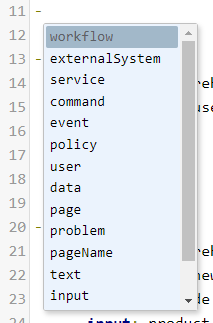
\includegraphics[width=4cm,height=6cm]{images/3.2/autocompletion-all} }}%
    \qquad
    \subfloat[\centering Mit Eingabe]{{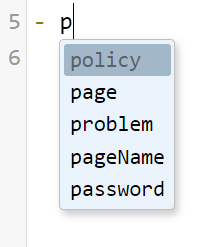
\includegraphics[width=4cm,height=5cm]{images/3.2/autocompletion-p} }}%
    \caption{Autovervollständigung}%
    \label{fig:autocompletion}%
\end{figure}

Dieses Add-On erstellt die in Abbildung~\ref{fig:autocompletion}((a)) angezeigt Liste.
Der Inhalt der Liste wird über ein in dieser Arbeit erstelltes Codemirror Add-On gefüllt.
Hierbei fällt auf, dass auch Schlüsselwörter angezeigt werden, welche nur im Kontext eines Page-Notes sinnvoll sind.
Das eigens geschriebene Add-On ist nicht kontextsensitiv und besitzt somit nicht die gleichen Funktionen wie die Autovervollständigung, welche eine IDE durch das JSON-Schema bereitstellt.
Der Code des geschriebenen Add-Ons befindet sich im Anhang dieser Arbeit, hierbei wird über die aktuelle Position des Cursors das aktuelle Wort extrahiert.
Damit ist es möglich über die Liste der Schlüsselwörter zu iterieren und zu prüfen, welche Vorschläge sinnvoll sind, sollte ein Wort bereits begonnen sein.
Dies ist anhand von Abbildung~\ref{fig:autocompletion}((b)) genauer zu erkennen.
Hierbei wurde bereits der Buchstabe \textit{p} eingetippt und das Add-On bietet zur Vervollständigung nur Wörter an, welche mit \textit{p} beginnen.

Des Weiteren wird durch das Betätigen der Tastenkombination ``Strg+S'' die Generierung angestoßen.
Bevor die Daten aus dem Codemirror zur Generierung an das Backend gesendet werden, werden diese auf Richtigkeit überprüft.
Da bereits ein JSON-Schema für fulibWorkflows existiert, wurde eine Bibliothek ausgewählt, welche einen Text über ein JSON-Schema validieren kann.
\textit{Ajv} ist ein solcher Validierungsmechanismus, allerdings kann mit Ajv lediglich ein JSON-Objekt mittels JSON-Schema validiert werden\cite*{ajv}.
Somit wurde zum Umwandeln des Textes aus dem Codemirror zu einem JSON-Objekt die Bibliothek \textit{js-yaml} verwendet\cite*{js-yaml}.

\begin{figure}[h]
    \centering
    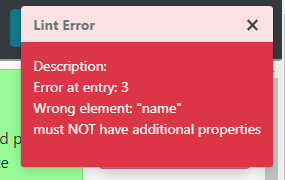
\includegraphics[width=0.4\textwidth]{images/3.2/error-toast}
    \caption{Validierungserror als Toast}
    \label{fig:error-toast}
\end{figure}

Sobald während der Validierung ein Problem mit der Eingabe erkannt wird, gibt diese einen Fehler zurück.
Dieser Fehler wird anschließend als Toast in der Oberfläche angezeigt, um den Nutzenden darauf hinzuweisen, an welcher Stelle die Eingabe im Codemirror nicht
dem JSON-Schema von fulibWorkflows entspricht.
Eine solche Fehlermeldung ist in Abbildung~\ref{fig:error-toast} dargestellt.
Hierbei wurde einem Note ein Attribut \textit{name} zugeordnet.
Da der besagte Note allerdings ein \textit{User} ist und im JSON-Schema festgelegt ist, dass ein User-Note keine zusätzlichen Attribute
besitzen darf, entsteht der in der Abbildung gezeigte Fehler.
Diese Fehlermeldung wird nach 20 Sekunden automatisch geschlossen.
Für die Darstellung von Toasts wurde die gleichnamige Komponente von \textit{ng-bootstrap} verwendet.
Sollte die Eingabe valide sein, so wird diese über einen Service an das Backend geschickt.

\subsection{Darstellung generierter Dateien}\label{subsec:darstellung-generierter-dateien}
Die anderen beiden Bereiche der Oberfläche, welche bisher nicht erläutert wurden, stellen jeweils einen bestimmten Teil der generierten Dateien dar.
Beide Bereiche aus Abbildung~\ref{fig:frontend} bestehen aus einem IFrame, wobei der obere IFrame das generierte \ac{ES}-Board anzeigt.
Andererseits übernimmt der untere IFrame die Anzeige der HTML-Mockups, den Objektdiagrammen und dem Klassendiagramm.

\begin{listing}[!ht]
    \inputminted{ts}{listings/3.2/GenerateResult.ts}
    \caption{Modell der vom Backend empfangenen Daten}
    \label{listing:generateResult}
\end{listing}

Bevor auf die Darstellung und Funktionen der IFrames eingegangen wird, wird zuerst betrachtet in welcher Form die generierten Dateien vom Backend im Frontend verarbeitet werden.
Die Form ist in Listing~\ref{listing:generateResult} dargestellt, in einem GenerateResult-Objekt werden alle generierten Dateien und Zusatzinformationen abgespeichert.
Bei den Zusatzinformationen handelt es sich um die Anzahl der generierten Diagramme und HTML-Mockups.
Die generierten Dateien werden als reiner String behandelt.
Um den Zugriff auf einzelne Objektdiagramme oder Mockups zu vereinfachen, sind diese jeweils in einer Map abgespeichert.
Bei den Maps ist jedem Diagramm/Mockup eine eindeutige Nummer zugeordnet.

Der obere IFrame erhält als Eingabe das \ac{ES}-Board und stellt dieses dar.
Dies ist möglich, da das \ac{ES}-Board eine valide HTML-Datei ist, welche durch einen IFrame dargestellt werden kann.
In Abbildung~\ref{fig:esBoard} ist ein \ac{ES}-Board für das im Web-Editor vorhandene Microservices-Beispiel dargestellt.

\begin{figure}[h]
    \centering
    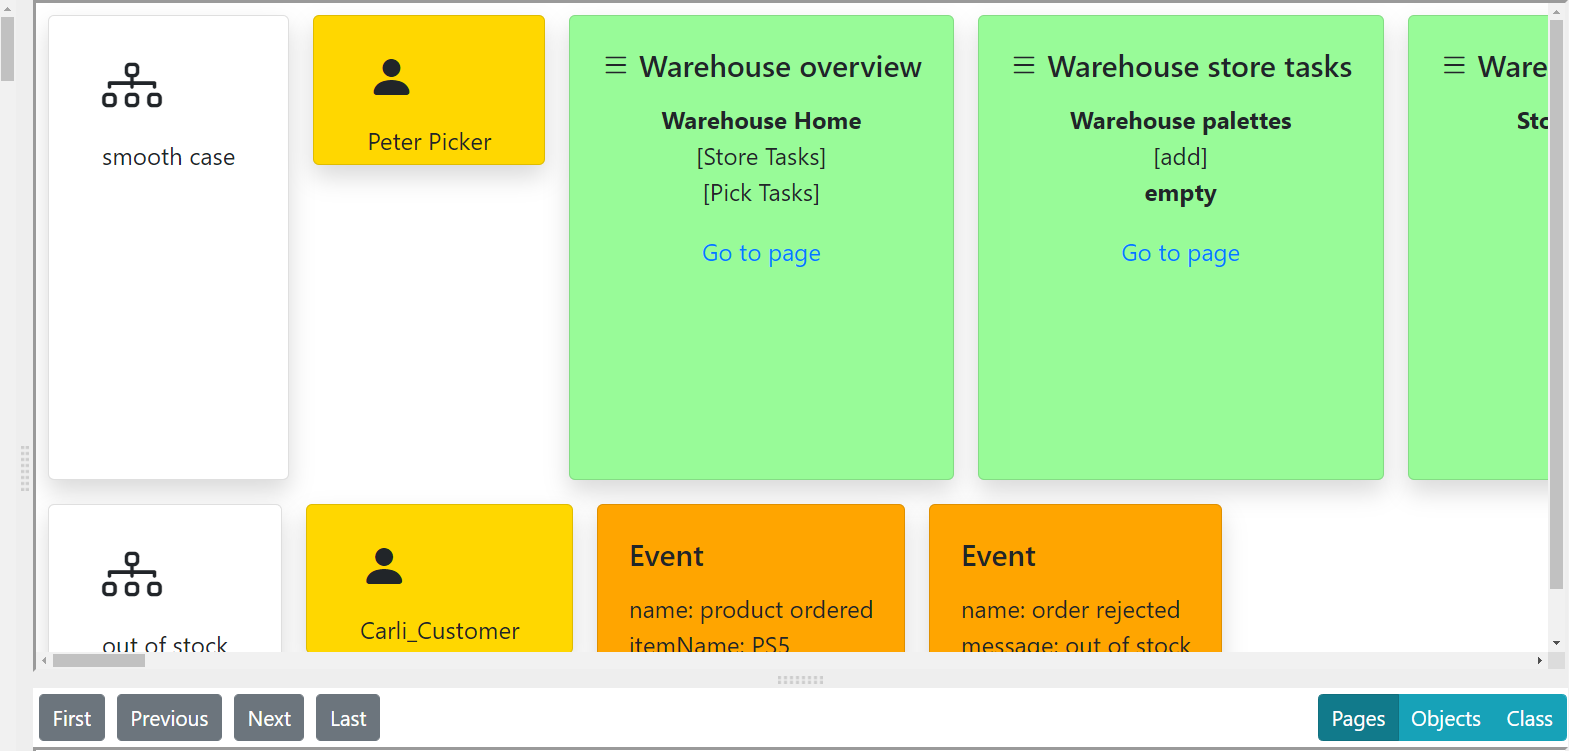
\includegraphics[width=1.0\textwidth]{images/3.2/board}
    \caption{Event-Storming-Board in einem IFrame}
    \label{fig:esBoard}
\end{figure}

Hierbei ist zu erwähnen, dass die Bereiche: Code-Editor, \ac{ES}-Board-IFrame und der IFrame zur Anzeige der Mockups und Diagramme beliebig vergrößert oder verkleinert werden kann.
Um dies zu ermöglichen wurde die Bibliothek \textit{angular-split} verwendet.
Diese ermöglicht es Bereiche zu definieren und darin Inhalt zu platzieren, sowie die Veränderung der Größen der Bereiche bereitzustellen\cite*{angular-split}.
Das Abändern der Größe von Bereichen ermöglicht das Hervorheben des Editors, des \ac{ES}-Boards oder der Mockups/Diagramme.

Für den unteren IFrame gelten die gleichen Gegebenheiten wie für den oberen IFrame.
Da es mehrere Mockups oder Diagramme geben kann, existieren vier Knöpfe, mit welchen es möglich ist zwischen den Mockups/Diagrammen zu wechseln.
Der Wechsel zwischen diesen Elementen ist nicht nur über die vier Knöpfe möglich, sondern ebenfalls über die entsprechenden Notes aus dem \ac{ES}-Board-IFrame.
Für jeden Page- oder Data-Note existiert in der Anzeige ein Link, welcher als Knopf fungiert, mit welchem zu dem Mockup oder Diagramm des Notes gewechselt werden kann.

Zuletzt existieren drei weitere Buttons auf Höhe der Buttons zum Wechseln der Page oder des Diagramms, welche die Anzeige der generierten Dateien manuell umschaltet,
dies ist ebenfalls in Abbildung~\ref{fig:frontend} dargestellt.
Hierbei kann zwischen dem Anzeigen der Mockups (Pages), der Objektdiagramme und des Klassendiagramms umgeschaltet werden.
